\chapter{畳み込み層並列化と相互通信についての検討}
\section{概要}
この章では、まず、マルチFiC-SW1システム上でCNNを扱うために畳み込み層の並列化を行う。
そして、その並列畳み込み演算をFiC-SW1上に実装した場合の相互通信について検討する。

\cite{fpgaopt}によれば、識別時において、畳み込み層での演算は全体の実行時間の90%以上を占めることがわかっている。
今回の実装では特にこの畳み込み演算をマルチFiC-SW1システムによって高速化することを重要な課題とした。

\section{畳み込み層の並列化}
畳み込み層の演算は多くの場合において、高いデータ並列性があるため、様々な並列化方式を考えることができる。

今回は、ほかの多くのニューラルネットアクセラレータ\cite{fpgaopt}\cite{dadiannao}と同様に、
入出力の特徴マップを相互通信し、重みデータをローカルストレージに保存する戦略をとった。
これは、特徴マップの計算量が(M×R×C)であるのに対して重みは(M×N×K×K)で、
一般的なCNNでは重みのほうが計算量が多くなる傾向があり、特徴マップを相互通信するほうが低コストになるからである。

図\ref{fig_paraconv}はCONV1を例に、今回の戦略で畳み込み層を16並列化したときのタスク分割の様子を示している。
AlexNetのCONV1は[3, 227, 227]のサイズの入力特徴マップから、[96, 3, 11, 11]のサイズの重みを用いて、
[96, 55, 55]のサイズの特徴マップを出力するものである。これを16並列化すると、重みが16分割されるため、1ノードあたりの
重みは[6, 3, 11, 11]となる。それに伴って、出力特徴マップのサイズも16分の1になるため、[6, 55, 55]となる。
ただし、この16分の1の出力は次の層のために全対全の相互通信によって共有しなければならない。

図\ref{fig_cnn_broadcast}はAlexNetを並列化した際に、どのタイミングで特徴マップ共有のための全対全通信が必要になるかを示している。
基本的には、ひとつの畳み込み層・識別層に対して1回の共有をしなければならない。また、正規化層の前でも共有が必要に
なるが、これはLRNの演算で使う前後2チャンネル分の特徴マップに対してのみであり、全対全通信と比べて遥かに小さいため、今回は詳しくは扱わない。

以下は、並列化された畳み込み演算を疑似コードで表したものになる。Tmの値によって並列度が変化し、たとえば、M=96のCONV1を16並列化
した場合、Tm=6となる。

\begin{itembox}[1]{出力特徴マップチャンネルで並列化された畳み込み演算のCコード}
\begin{verbatim}
for (int tr = 0; tr < R; tr++)
  for (int tc = 0; tc < C; tc++)
    for (int to = 0; to < M; to += Tm) //Tmごとに出力を分割
      for (int ti = 0; ti < N; ti++)
        for (int i = 0; i < K; i++)
          for (int j = 0; j < K; j++)
            output[to][tr][tc] +=
              input[ti][S*tr+i][S*tc+j] *
              weight[to][ti][i][j];
\end{verbatim}
\end{itembox}
						
						
\begin{figure}[ht]  
 \begin{center}   
	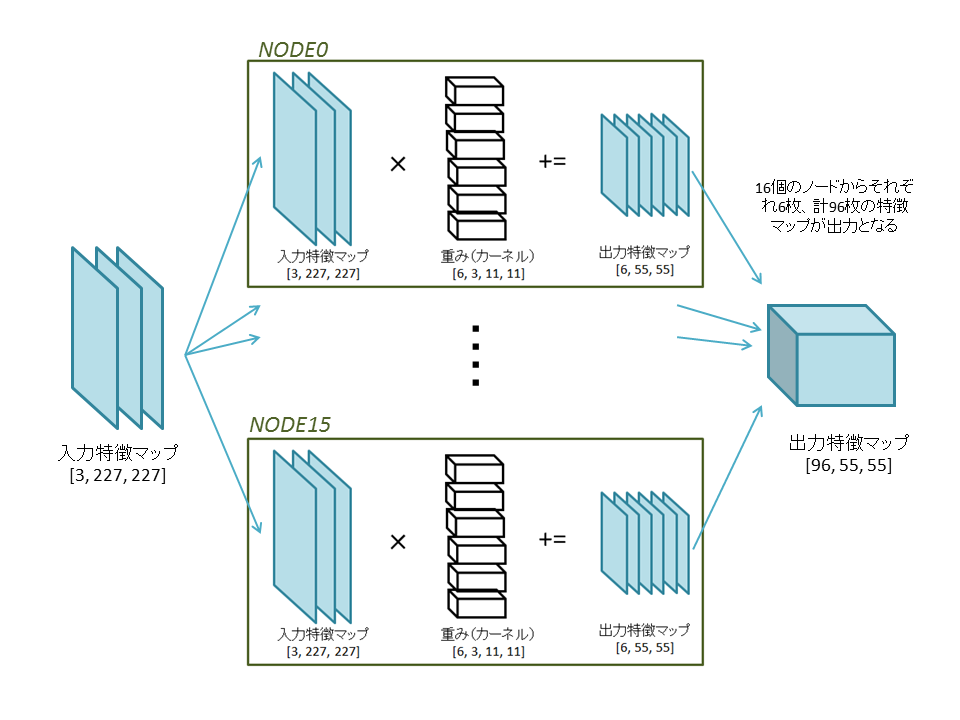
\includegraphics[width=1.0\columnwidth,bb=0 0 720 540]{img/paraconv.png}
  \caption{16並列化されたCONV1の畳み込み演算の例}
%  \ecaption{Static analysis result of an example pattern}
  \label{fig_paraconv}  
 \end{center}  
\end{figure}

\begin{figure}[ht]  
 \begin{center}   
	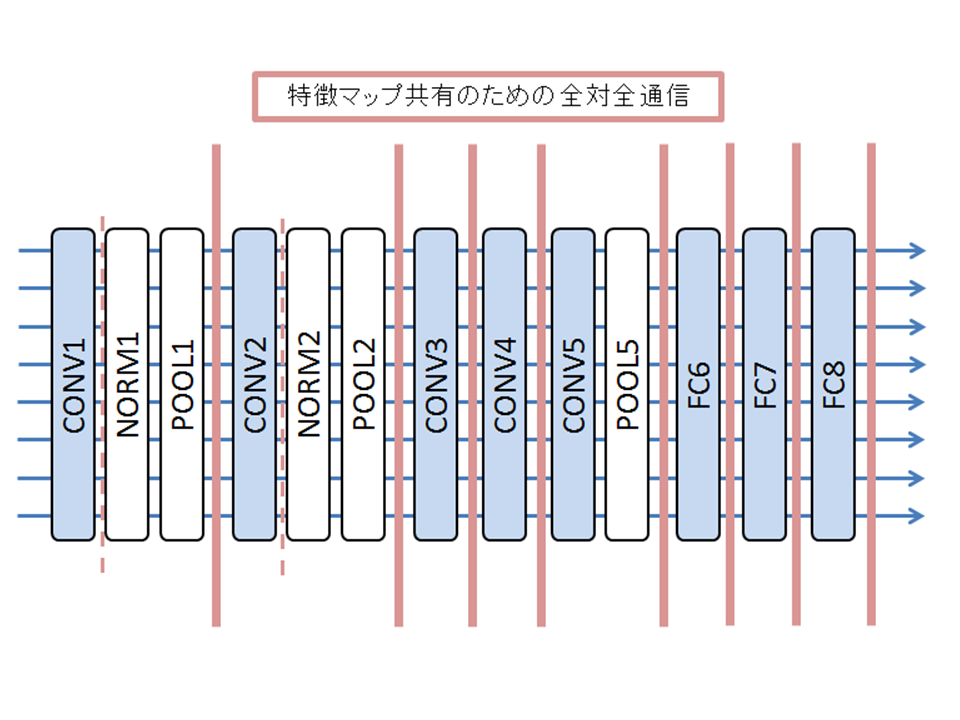
\includegraphics[width=1.0\columnwidth,bb=0 0 720 540]{img/cnn_broadcast.png}
  \caption{並列化されたAlexNetにおける特徴マップ共有のタイミング}
%  \ecaption{Static analysis result of an example pattern}
  \label{fig_cnn_broadcast}  
 \end{center}  
\end{figure}

\section{マルチFiC-SW1システム上での並列化された畳み込み層の扱い}
さて、並列畳み込み演算をマルチFiC-SW1システム上での処理に置き換えると、1ノードをひとつのFiC-SW1ボードに置き換えるのが妥当である。
重みはFiC-SW1上のFPGAのメモリ資源かDRAMをローカルストレージとして用いて保存する。
また、入出力特徴マップのためもバッファを設けて、必要に応じてサーキットスイッチネットワークを利用してブロードキャストする形になる。

図\ref{fig_cnn_on_sw1}はFiC-SW1ボード上での畳み込み層の演算について解説している。
まず、演算に必要な入力特徴マップがブロードキャストによって送信されてくるまで待機しなければならない。
データが揃ったならローカルストレージの重みを用いて畳み込み演算を行い、その間はサーキットスイッチからは空データを受信し続ける。
計算が終わったら、その出力特徴マップをブロードキャストする。すべてのFiC-SW1は基本的には非同期的に動作するが、
すべてのノードがブロードキャストし終えないと次の層の処理を始めることができないため、このタイミングで同期が取られる。

さて、表\ref{node}に、このシステムでAlexNetを実装した際のひとつのFiC-SW1あたりの出力特徴マップ数とブロードキャストされるデータ量を
算出した結果を示す。並列度が高くなるほど1ノードが扱う出力特徴マップ数が減っていることがわかる。しかし、たとえば、CONV1の結果を見ると、
16並列から64並列では並列度は4倍になっているのに対して、出力特徴マップ数は6チャンネルから2チャンネルと4分の1にはなっていない。
CONV1の出力特徴マップ数96は、64で割り切れないため、最適なタスク分割を行えていないことが理由である。
このように畳み込み層の出力特徴マップ数によっては、過剰な並列化は通信の無駄を増やしてしまうことに注意しなければならない。

\begin{figure}[ht]  
 \begin{center}   
	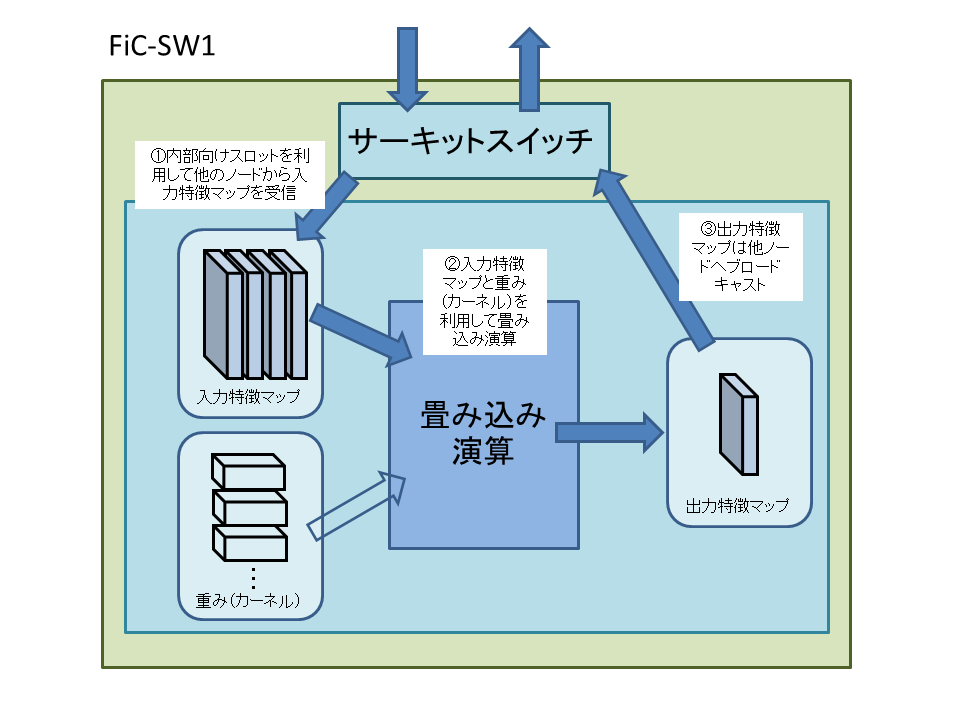
\includegraphics[width=1.0\columnwidth,bb=0 0 720 540]{img/cnn_on_sw1.png}
  \caption{FiC-SW1上のCNNの計算処理の流れ}
%  \ecaption{Static analysis result of an example pattern}
  \label{fig_cnn_on_sw1}  
 \end{center}  
\end{figure}

\begin{table}[ht]
 \begin{center}
  \caption{マルチノードCNNの1ノードあたりの出力特徴マップ数とそのデータ量}
   \begin{tabular}{|c|c|c|c|c|c|c|c|c|} \hline
     & \multicolumn{2}{|c|}{4並列} & \multicolumn{2}{c|}{16並列} & \multicolumn{2}{c|}{64並列} & \multicolumn{2}{c|}{265並列}\\ \hline
     & fm & (Kb) & fm & (Kb) & fm & (Kb) & fm & (Kb) \\ \hline
     CONV1 & 24 & 559.9 & 6 & 140.0 & 2 & 46.6 & 1 & 23.3 \\
     CONV2 & 64 & 346.1 & 16 & 86.5 & 4 & 21.6 & 1 & 5.4 \\
     CONV3 & 96 & 519.2 & 24 & 129.8 & 6 & 32.4 & 2 & 10.8 \\
     CONV4 & 96 & 519.2 & 24 & 129.8 & 6 & 32.4 & 2 & 10.8 \\
     CONV5 & 64 & 73.7 & 16 & 18.4 & 4 & 4.6 & 1 & 1.2 \\
     FC6 & 1024 & 32.8 & 256 & 8.2 & 64 & 2.0 & 16 & 0.5 \\
     FC7 & 1024 & 32.8 & 256 & 8.2 & 64 & 2.0 & 16 & 0.5 \\
     FC8 & 250 & 8.0 & 63 & 2.0 & 16 & 0.5 & 4 & 0.1 \\ \hline
  \end{tabular}
  \label{node}  
 \end{center}
\end{table}

\section{FiC-SW1ネットワークによる特徴マップ共有}
図\ref{gra_broadcast_time}は、表\ref{node}を基に、出力特徴マップをFiC-SW1の時分割多重のサーキットスイッチネットワークによって
共有した場合の通信時間の予測を示す。表\ref{tdmtime}は図\ref{gra_broadcast_time}の詳細をまとめたものである。
出力特徴マップのサイズ(R、C)が他の層と比べて大きいCONV1では16並列時で
699.84$\mu$secの通信時間が発生するが、特徴マップのサイズが小さくなるにつれ減少していき、最後のFC8では10.08$\mu$secとなる。
この計算では、FiC-SW1のサーキットスイッチのスロットひとつに、ひとつの特徴マップの値を格納した場合を仮定している。
実際のFiC-SW1のスロットは80bit程度になるので32bit浮動小数点数データを2つ格納できる可能性が高いが、今回はアクセラレータに
合わせて1サイクルにつきデータひとつの場合を扱った。

時分割多重方式による通信ではノード数が増えるほど通信帯域が狭くなるが、
今回のシステムではそのノード数が増えれば1ノードあたりの送信量も減るため、結果としてノード数に対して依存しにくい通信時間となる。
しかし、表\ref{node}に見られるように、過剰な並列度では最適なタスク分割を行うことができず、通信帯域を狭めるだけになってしまい
共有にかかる時間コストが増大してしまう。

これらの結果は、すべてのノードが16Gbps(8Gbps全二重)の通信路を最大限利用できたときの、理想的状態を仮定したときのものである。
また、ネットワークのトポロジ、通信遅延などは考慮していない。
これらを含めた通信時間予測は今後の課題とするが、このような要因によって通信時間は今回の結果より大きくなってしまうことが予想される。

\begin{figure}[ht]  
 \begin{center}   
	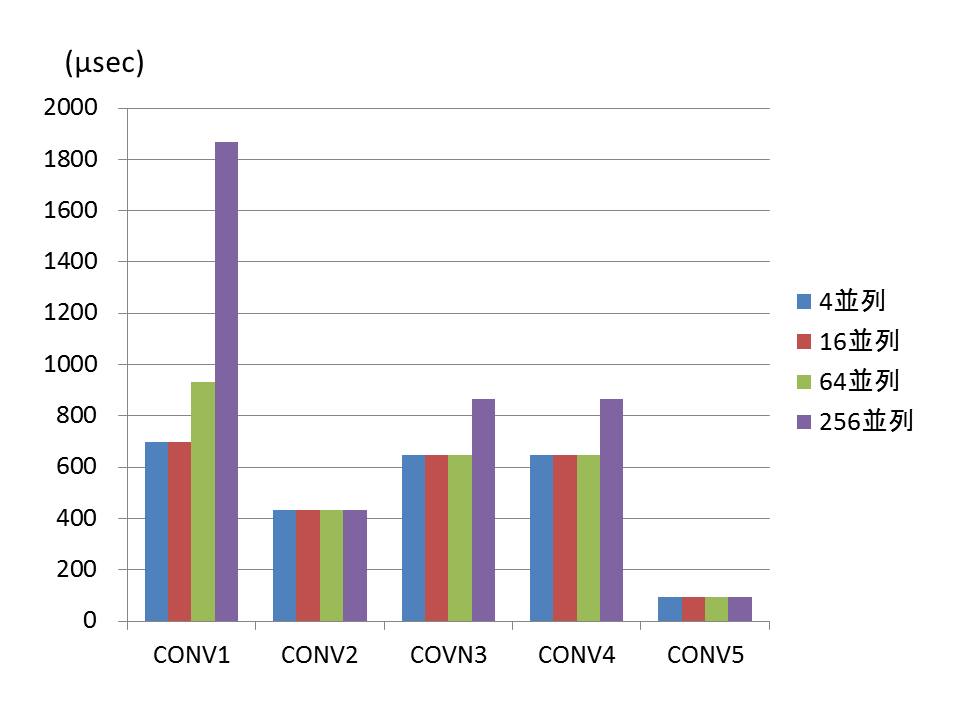
\includegraphics[width=1.0\columnwidth,bb=0 0 720 540]{img/broadcast_time.png}
  \caption{畳み込み層の特徴マップ共有にかかる通信時間($\mu$sec)の予測}
%  \ecaption{Static analysis result of an example pattern}
  \label{gra_broadcast_time}  
 \end{center}  
\end{figure}

\begin{table}[ht]
 \begin{center}
  \caption{特徴マップ共有の予測通信時間($\mu$sec)}
   \begin{tabular}{|c|c|c|c|c|} \hline
     層 & 4並列 & 16並列 & 64並列 & 256並列 \\ \hline
     CONV1 & 699.84 & 699.84 & 933.12 & 1866.24 \\
     CONV2 & 432.64 & 432.649 & 432.64 & 432.64 \\
     CONV3 & 648.96 & 648.96 & 648.96 & 865.28 \\
     CONV4 & 648.96 & 648.96 & 648.96 & 865.28 \\
     CONV5 & 92.16 & 92.16 & 92.16 & 92.16 \\
     FC6 & 40.96 & 40.96 & 40.96 & 40.96\\
     FC7 & 40.96 & 40.96 & 40.96 & 40.96\\
     FC8 & 10.00 & 10.08 & 10.24 & 10.24\\ \hline
  \end{tabular}
  \label{tdmtime}  
 \end{center}
\end{table}

\section{FiC-SW1ネットワークの通信帯域改善のための手法}
STDMによるサーキットスイッチングネットワークでは、通信の帯域を保証できるというメリットがあるが、ノード数が増えると
1ノードに与えられる通信帯域が極端に狭くなってしまうという問題が発生する。

時分割多重のスロット数を減らすことができれば、1スロットを複数のノードで共有する方針で、帯域を改善させることができる。
その単純な方法としては、データのヘッダ情報として、ラベルを定義する方法がある。
スロットを共有しているノードにはそれぞれ固有のラベル番号を振り、送信の際には自身のラベル番号と共にデータを送信するように設計することで、
帯域を狭めることなく疑似的にスロット数を増やすことが可能である。ただし、この帯域の改善方法では
1ノードがスロットを占有している間、そのスロットを共有している他のノードは送信を行うことができない。
そのため、各ノードのスロット占有時間が短い場合でないと有効に働かないと考えられる。
